\section{Numerical experiments}

\begin{frame}[t]\frametitle{Numerical experiments}
	Given $A$ and $B$ two $m\times n$ matrices, with $m\geq n$, and $c\in\mathbb{R}$, we consider the matrix function $f:\mathbb{R}^{n\times n}\to\mathbb{R}$ given by:
	$$f(X):=\dfrac{1}{2}\|AX-B\|^2_F + \sum_{i=1}^{n-1} \left[ c \left( X_{i+1,i+1}-X_{i,i}^2 \right)^2 + (1-X_{i,i})^2   \right],$$
	which combines a least squares term with a \textcolor{purple}{Rosenbrock-type} function. $X_{i,j}$ stands for the $ij$-element of the matrix $X$ and $\|\cdot\|_F$ denotes the Frobenius matrix norm, i.e., $\|A\|_F:=\sqrt{\langle A,A \rangle}$ where the inner product is given by $\langle A,B \rangle = \tr(A^TB)$.
\end{frame}


\begin{frame}[t]\frametitle{Numerical experiments}
	\begin{block}{Problem I\footfullcite{BirginMartinezRaydan2003}:}
		\begin{equation*}
			\begin{array}{cl}
				\displaystyle\min & f(X)           \\
				\mbox{s.t.}       & X \in SDD^+,   \\
				                  & L\leq X\leq U,
			\end{array}
		\end{equation*}
		where $SDD^+$ is the cone of \textcolor{purple}{symmetric and diagonally dominant real matrices with positive diagonal}, i.e.,
		\begin{equation}
			SDD^+ :=\{X\in\mathbb{R}^{n\times n}\mid X=X^T, \; X_{i,i}\geq \displaystyle\sum_{j\neq i}|X_{i,j}| \; \forall i\},
		\end{equation}
		$L$ and $U$ are given $n\times n$ matrices, and  $L\leq X\leq U$ means that $L_{i,j} \leq X_{i,j} \leq U_{i,j}$ for all $i,j$.
	\end{block}

	For Problem~I, we used the \textcolor{purple}{Dykstra's algorithm} described in \cite{BirginMartinezRaydan2003}, see also \cite{dykstraSDD} to compute the inexact projection. In this case, $SDD^+=\ds\cap_{i=1}^n SDD^+_i$, where

	\begin{equation}
		SDD^+_i :=\{X\in\R^{n\times n}\mid X=X^T, \; X_{i,i}\geq \ds\sum_{j\neq i}|X_{i,j}| \} \; \mbox{for all} \; i=1,\ldots,n.
	\end{equation}
\end{frame}


\begin{frame}[t]\frametitle{Numerical experiments}
	\begin{block}{Problem II\footfullcite{allen2017linear}\footfullcite{douglasprojected}:}
		\begin{equation*}
			\begin{array}{cl}
				\displaystyle\min & f(X)                  \\
				\mbox{s.t.}       & X \in \mathbb{S}^n_+, \\
				                  & \tr(X)=1,
			\end{array}
		\end{equation*}
		where $\mathbb{S}^n_+$ is the cone of \textcolor{purple}{symmetric and positive semidefinite real matrices}. The feasible set of Problem II was known as \textcolor{purple}{{\it spectrahedron}} and appears in several interesting applications.
	\end{block}

	We considered a variant of the \textcolor{purple}{Frank-Wolfe algorithm} proposed in \cite{allen2017linear}, which improves the convergence rate and the total time complexity of the classical Frank-Wolfe method. This algorithm specialized for the projection problem over the spectrahedron is carefully described in \cite{aguiar2021inexact}.
\end{frame}


\begin{frame}[t]\frametitle{Numerical experiments}

	We are interested in the \textcolor{purple}{spectral gradient version of the SPG method}, so we set $D_k:=I$ for all $k$, $\alpha_0 := \min(\alpha_{\max}, \max(\alpha_{\min}, 1/ \| \nabla f(x^0) \|))$ and, for $k>0$,

	\begin{equation}
		\alpha_k:=\left\{
		\begin{array}{ll}
			\displaystyle\min (\alpha_{\max},\max (\alpha_{\min},\langle s^k,s^k\rangle/\langle s^k,y^k\rangle)), & \mbox{if} \; \langle s^k,y^k\rangle > 0 \\
			\alpha_{\max},                                                                                        & \mbox{otherwise},
		\end{array}\right.
	\end{equation}
	where $s^k:=X^k - X^{k-1}$, $y^k:=\nabla f(X^k) - \nabla f(X^{k-1})$, $\alpha_{\min}=10^{-10}$, and $\alpha_{\max}=10^{10}$.


	Concerning the stopping criterion, all runs were stopped at an iterate $X^k$ declaring convergence if
	$$
		\displaystyle \max_{i,j} (|X^k_{i,j}-W^k_{i,j}| )\leq 10^{-6},
	$$
	where $W^k \in {\cal P}_{C, \zeta_k}^{D_k}(x^{k}, z^k)$.
\end{frame}


\begin{frame}[t]\frametitle{Influence of the inexact projection}
	\begin{figure}[H]\centering
		\begin{tabular}{ccc}
			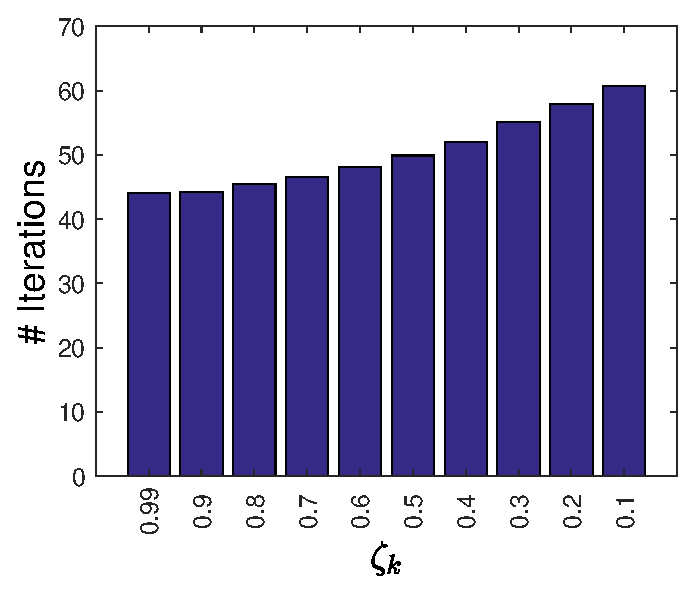
\includegraphics[scale=\myscaleF]{../figures/SDDit} & 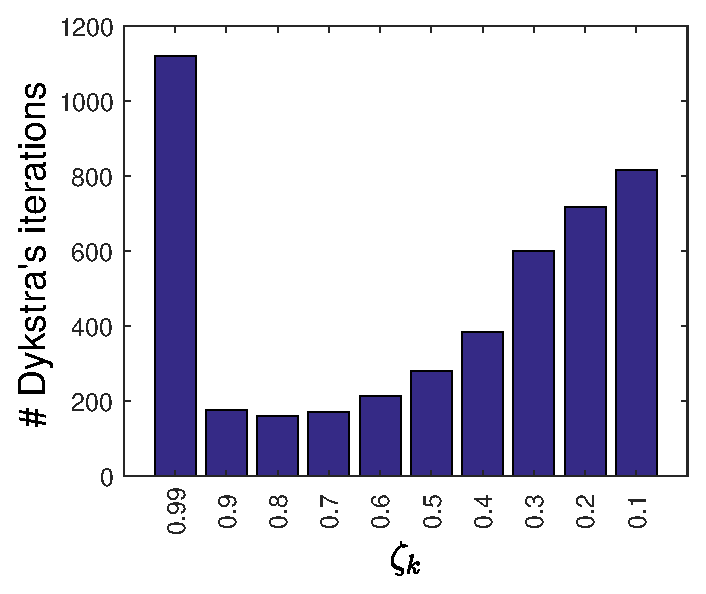
\includegraphics[scale=\myscaleF]{../figures/SDDDIT} & \includegraphics[scale=\myscaleF]{../figures/SDDtime} \\
			(a)                                                 & (b)                                                  & (c)                                                   \\
		\end{tabular}
		\caption{Results for 10 instances of Problem I using $n=100$, $m=200$, and $c=10$. Average number of: (a) iterations; (b) Dykstra’s iterations; (c)  CPU time in seconds needed to reach the solution for different choices of $\zeta_k$.}
	\end{figure}
\end{frame}

\begin{frame}[t]\frametitle{Influence of the inexact projection}
	\begin{figure}[H]\centering
		\begin{tabular}{ccc}
			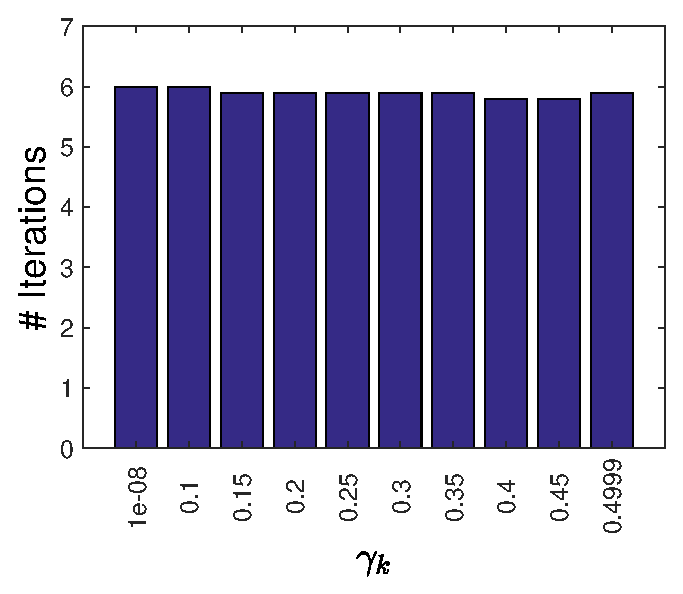
\includegraphics[scale=\myscaleF]{../figures/Specit} & 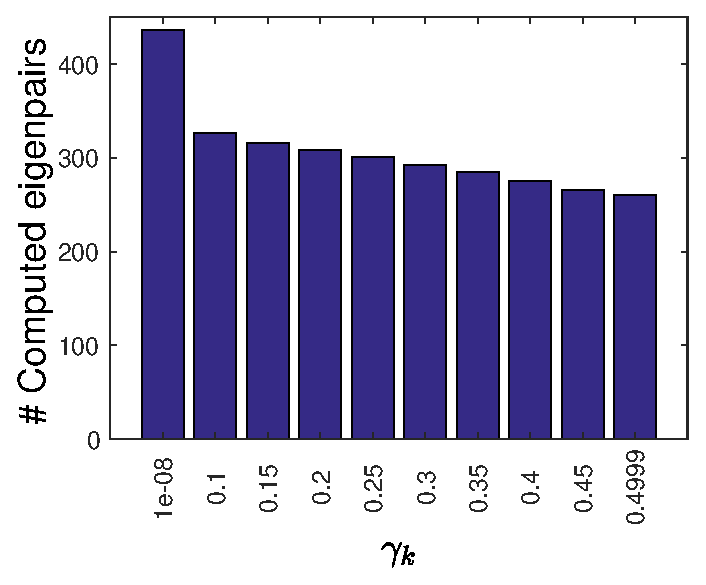
\includegraphics[scale=\myscaleF]{../figures/SpecFWIT} & \includegraphics[scale=\myscaleF]{../figures/Spectime} \\
			(a)                                                  & (b)                                                    & (c)                                                    \\
		\end{tabular}
		\caption{Results for 10 instances of Problem II using $n=800$, $m=1000$, and $c=100$. Average number of: (a) iterations; (b) computed eigenpairs; (c)  CPU time in seconds needed to reach the solution for different choices of $\gamma_k$.}
	\end{figure}
\end{frame}

\begin{frame}[t]\frametitle{Influence of the line search scheme}

	\begin{figure}[H]\centering
		\begin{tabular}{cccc}
			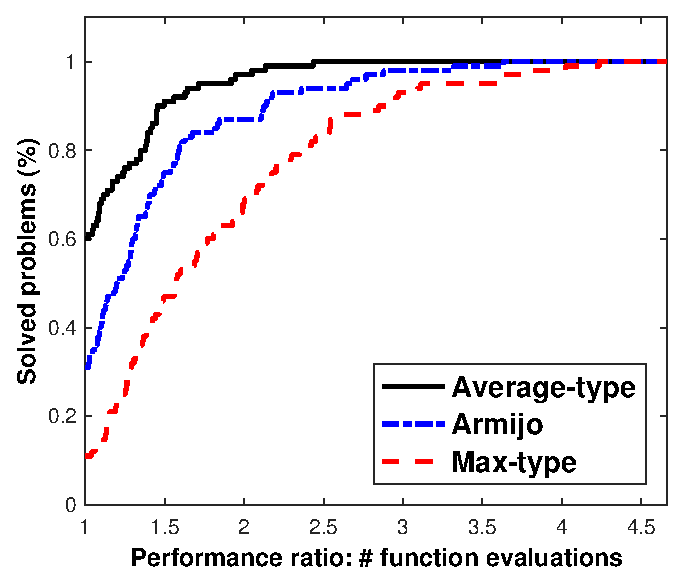
\includegraphics[scale=\myscale]{../figures/ppSDDnfev} & 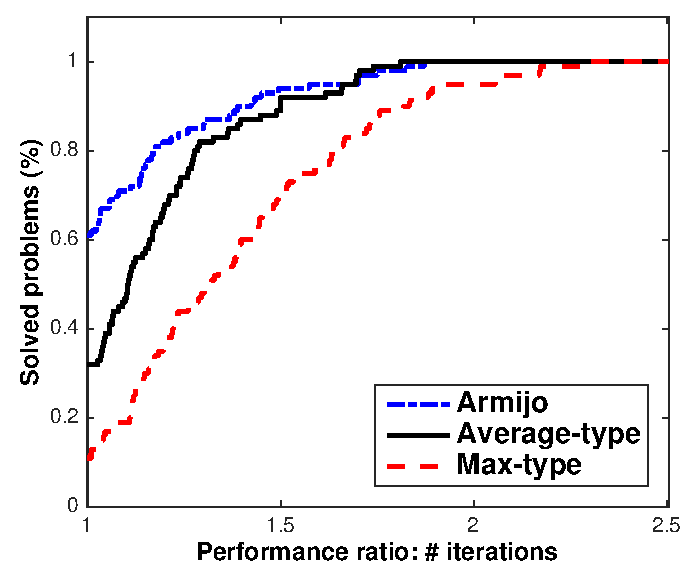
\includegraphics[scale=\myscale]{../figures/ppSDDit} & 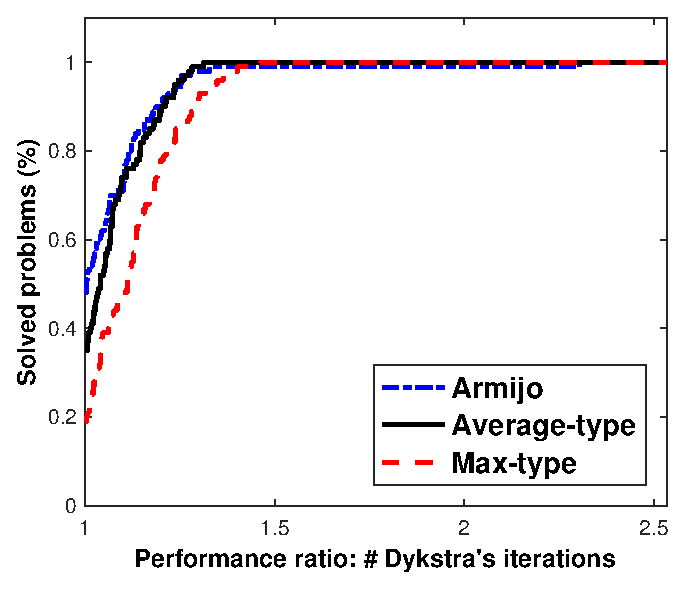
\includegraphics[scale=\myscale]{../figures/ppSDDnDIT} & 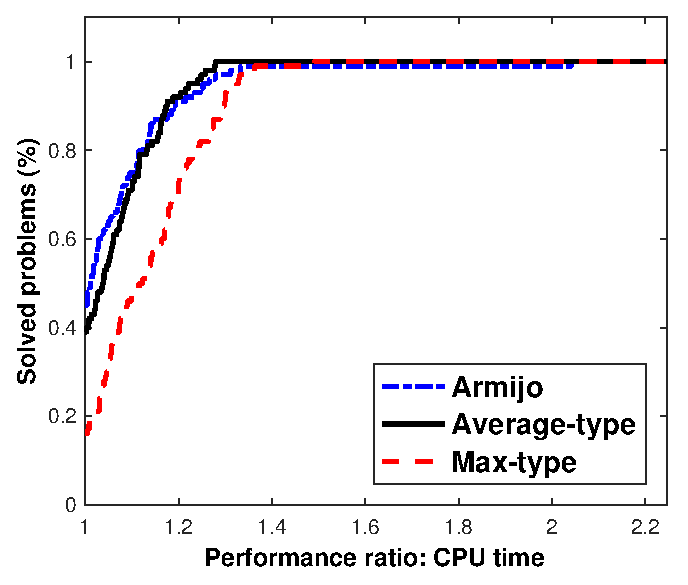
\includegraphics[scale=\myscale]{../figures/ppSDDtime} \\
			(a)                                                    & (b)                                                  & (c)                                                    & (d)                                                    \\
		\end{tabular}
		\caption{Performance profiles for Problem~I considering the SPG method with the Armijo, the Average-type, and the Max-type line searches strategies using as performance measurement: (a) number of function evaluations; (b) number of (outer) iterations; (c) number of Dykstra’s iterations; (d) CPU time.}

	\end{figure}
\end{frame}

\begin{frame}[t]\frametitle{Influence of the line search scheme}
	\begin{figure}[H]\centering
		\begin{tabular}{cccc}
			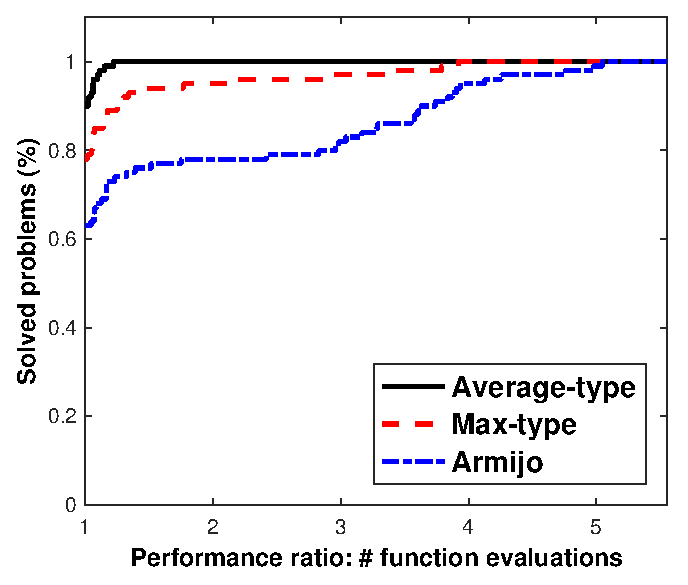
\includegraphics[scale=\myscale]{../figures/ppSpecnfev} & 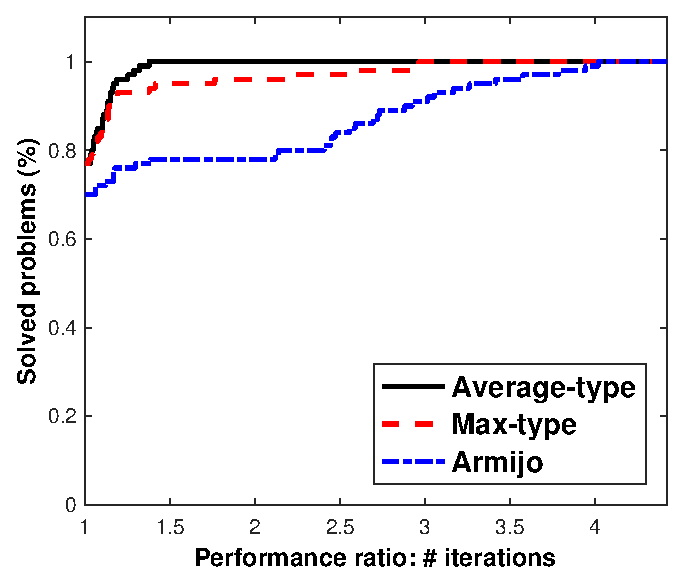
\includegraphics[scale=\myscale]{../figures/ppSpecit} & 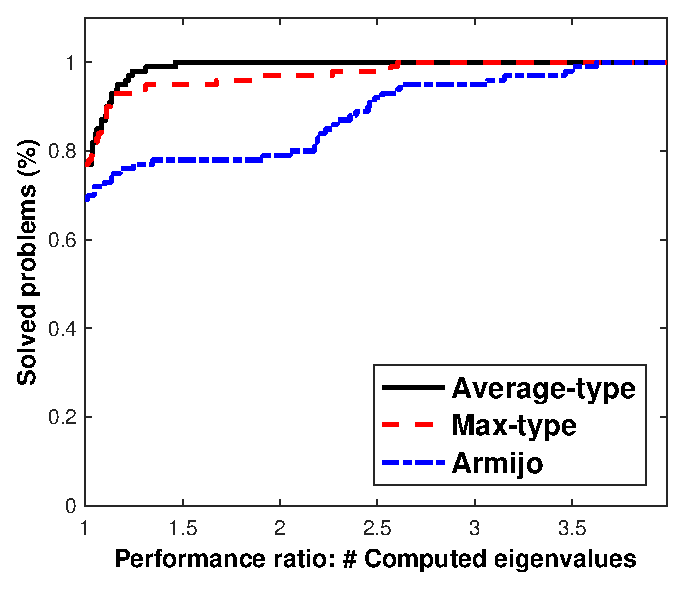
\includegraphics[scale=\myscale]{../figures/ppSpecnFW} & 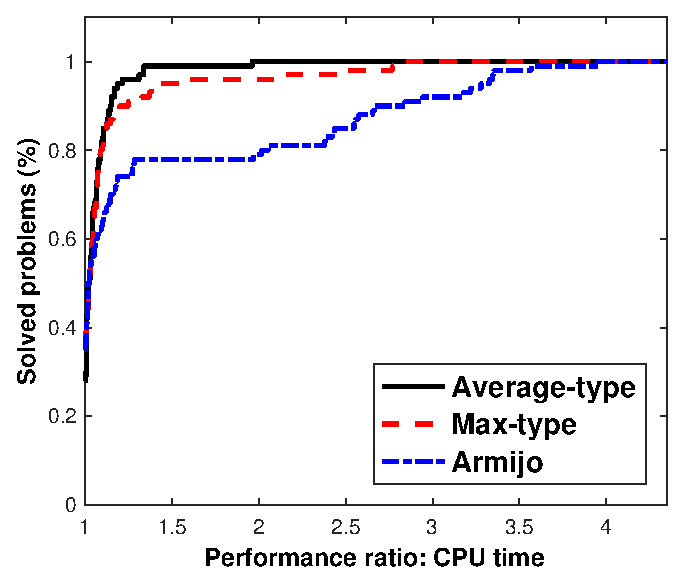
\includegraphics[scale=\myscale]{../figures/ppSpectime} \\
			(a)                                                     & (b)                                                   & (c)                                                    & (d)                                                     \\
		\end{tabular}
		\caption{Performance profiles for Problem~II considering the SPG method with the Armijo, the Average-type, and the Max-type line searches strategies using as performance measurement: (a) number of function evaluations; (b) number of (outer) iterations; (c) number of computed eigenpairs; (d) CPU time.}
	\end{figure}
\end{frame}